% Options for packages loaded elsewhere
\PassOptionsToPackage{unicode}{hyperref}
\PassOptionsToPackage{hyphens}{url}
%
\documentclass[
]{article}
\usepackage{lmodern}
\usepackage{amssymb,amsmath}
\usepackage{ifxetex,ifluatex}
\ifnum 0\ifxetex 1\fi\ifluatex 1\fi=0 % if pdftex
  \usepackage[T1]{fontenc}
  \usepackage[utf8]{inputenc}
  \usepackage{textcomp} % provide euro and other symbols
\else % if luatex or xetex
  \usepackage{unicode-math}
  \defaultfontfeatures{Scale=MatchLowercase}
  \defaultfontfeatures[\rmfamily]{Ligatures=TeX,Scale=1}
\fi
% Use upquote if available, for straight quotes in verbatim environments
\IfFileExists{upquote.sty}{\usepackage{upquote}}{}
\IfFileExists{microtype.sty}{% use microtype if available
  \usepackage[]{microtype}
  \UseMicrotypeSet[protrusion]{basicmath} % disable protrusion for tt fonts
}{}
\makeatletter
\@ifundefined{KOMAClassName}{% if non-KOMA class
  \IfFileExists{parskip.sty}{%
    \usepackage{parskip}
  }{% else
    \setlength{\parindent}{0pt}
    \setlength{\parskip}{6pt plus 2pt minus 1pt}}
}{% if KOMA class
  \KOMAoptions{parskip=half}}
\makeatother
\usepackage{xcolor}
\IfFileExists{xurl.sty}{\usepackage{xurl}}{} % add URL line breaks if available
\IfFileExists{bookmark.sty}{\usepackage{bookmark}}{\usepackage{hyperref}}
\hypersetup{
  pdftitle={Logistic Regession},
  pdfauthor={F.A. Barrios},
  hidelinks,
  pdfcreator={LaTeX via pandoc}}
\urlstyle{same} % disable monospaced font for URLs
\usepackage[margin=1in]{geometry}
\usepackage{color}
\usepackage{fancyvrb}
\newcommand{\VerbBar}{|}
\newcommand{\VERB}{\Verb[commandchars=\\\{\}]}
\DefineVerbatimEnvironment{Highlighting}{Verbatim}{commandchars=\\\{\}}
% Add ',fontsize=\small' for more characters per line
\usepackage{framed}
\definecolor{shadecolor}{RGB}{248,248,248}
\newenvironment{Shaded}{\begin{snugshade}}{\end{snugshade}}
\newcommand{\AlertTok}[1]{\textcolor[rgb]{0.94,0.16,0.16}{#1}}
\newcommand{\AnnotationTok}[1]{\textcolor[rgb]{0.56,0.35,0.01}{\textbf{\textit{#1}}}}
\newcommand{\AttributeTok}[1]{\textcolor[rgb]{0.77,0.63,0.00}{#1}}
\newcommand{\BaseNTok}[1]{\textcolor[rgb]{0.00,0.00,0.81}{#1}}
\newcommand{\BuiltInTok}[1]{#1}
\newcommand{\CharTok}[1]{\textcolor[rgb]{0.31,0.60,0.02}{#1}}
\newcommand{\CommentTok}[1]{\textcolor[rgb]{0.56,0.35,0.01}{\textit{#1}}}
\newcommand{\CommentVarTok}[1]{\textcolor[rgb]{0.56,0.35,0.01}{\textbf{\textit{#1}}}}
\newcommand{\ConstantTok}[1]{\textcolor[rgb]{0.00,0.00,0.00}{#1}}
\newcommand{\ControlFlowTok}[1]{\textcolor[rgb]{0.13,0.29,0.53}{\textbf{#1}}}
\newcommand{\DataTypeTok}[1]{\textcolor[rgb]{0.13,0.29,0.53}{#1}}
\newcommand{\DecValTok}[1]{\textcolor[rgb]{0.00,0.00,0.81}{#1}}
\newcommand{\DocumentationTok}[1]{\textcolor[rgb]{0.56,0.35,0.01}{\textbf{\textit{#1}}}}
\newcommand{\ErrorTok}[1]{\textcolor[rgb]{0.64,0.00,0.00}{\textbf{#1}}}
\newcommand{\ExtensionTok}[1]{#1}
\newcommand{\FloatTok}[1]{\textcolor[rgb]{0.00,0.00,0.81}{#1}}
\newcommand{\FunctionTok}[1]{\textcolor[rgb]{0.00,0.00,0.00}{#1}}
\newcommand{\ImportTok}[1]{#1}
\newcommand{\InformationTok}[1]{\textcolor[rgb]{0.56,0.35,0.01}{\textbf{\textit{#1}}}}
\newcommand{\KeywordTok}[1]{\textcolor[rgb]{0.13,0.29,0.53}{\textbf{#1}}}
\newcommand{\NormalTok}[1]{#1}
\newcommand{\OperatorTok}[1]{\textcolor[rgb]{0.81,0.36,0.00}{\textbf{#1}}}
\newcommand{\OtherTok}[1]{\textcolor[rgb]{0.56,0.35,0.01}{#1}}
\newcommand{\PreprocessorTok}[1]{\textcolor[rgb]{0.56,0.35,0.01}{\textit{#1}}}
\newcommand{\RegionMarkerTok}[1]{#1}
\newcommand{\SpecialCharTok}[1]{\textcolor[rgb]{0.00,0.00,0.00}{#1}}
\newcommand{\SpecialStringTok}[1]{\textcolor[rgb]{0.31,0.60,0.02}{#1}}
\newcommand{\StringTok}[1]{\textcolor[rgb]{0.31,0.60,0.02}{#1}}
\newcommand{\VariableTok}[1]{\textcolor[rgb]{0.00,0.00,0.00}{#1}}
\newcommand{\VerbatimStringTok}[1]{\textcolor[rgb]{0.31,0.60,0.02}{#1}}
\newcommand{\WarningTok}[1]{\textcolor[rgb]{0.56,0.35,0.01}{\textbf{\textit{#1}}}}
\usepackage{graphicx,grffile}
\makeatletter
\def\maxwidth{\ifdim\Gin@nat@width>\linewidth\linewidth\else\Gin@nat@width\fi}
\def\maxheight{\ifdim\Gin@nat@height>\textheight\textheight\else\Gin@nat@height\fi}
\makeatother
% Scale images if necessary, so that they will not overflow the page
% margins by default, and it is still possible to overwrite the defaults
% using explicit options in \includegraphics[width, height, ...]{}
\setkeys{Gin}{width=\maxwidth,height=\maxheight,keepaspectratio}
% Set default figure placement to htbp
\makeatletter
\def\fps@figure{htbp}
\makeatother
\setlength{\emergencystretch}{3em} % prevent overfull lines
\providecommand{\tightlist}{%
  \setlength{\itemsep}{0pt}\setlength{\parskip}{0pt}}
\setcounter{secnumdepth}{-\maxdimen} % remove section numbering

\title{Logistic Regession}
\author{F.A. Barrios}
\date{2020-11-28}

\begin{document}
\maketitle

\begin{Shaded}
\begin{Highlighting}[]
\CommentTok{# All the needed libraries}
\KeywordTok{library}\NormalTok{(tidyverse)}
\KeywordTok{library}\NormalTok{(emmeans)}
\KeywordTok{library}\NormalTok{(wesanderson)}
\KeywordTok{library}\NormalTok{(rstatix)}
\KeywordTok{library}\NormalTok{(HSAUR2)}
\KeywordTok{library}\NormalTok{(car)}
\KeywordTok{library}\NormalTok{(effects)}

\KeywordTok{setwd}\NormalTok{(}\StringTok{"~/Dropbox/GitHub/Class2020"}\NormalTok{)}
\NormalTok{wcgs <-}\StringTok{ }\KeywordTok{read_csv}\NormalTok{(}\StringTok{"DataRegressBook/Chap2/wcgs.csv"}\NormalTok{)}
\end{Highlighting}
\end{Shaded}

\hypertarget{examples-from-the-car-book-fox-weisberg-1}{%
\section[Examples from the CAR book (Fox \& Weisberg)
]{\texorpdfstring{Examples from the CAR book (Fox \& Weisberg)
\footnote{All notes are taken form the ``Companion to Applied
  Regression'', 3rd Ed. Fox \& Weisberg}}{Examples from the CAR book (Fox \& Weisberg) }}\label{examples-from-the-car-book-fox-weisberg-1}}

\hypertarget{review-of-the-structure-of-glms}{%
\subsection{Review of the Structure of
GLMs}\label{review-of-the-structure-of-glms}}

The structure of a GLM is very similar to that of the linear model. In
particular we have a response variable \emph{y} and \emph{k} predictors,
and we are interested in understanding how the mean of \emph{y} varies
as the values of the predictors change.

A GLM consists of three components

\begin{enumerate}
\def\labelenumi{\arabic{enumi}.}
\item
  Random component, specifying the conditional or ``error'' distribution
  of the response variable, \(y\), given the predictors from an
  \emph{exponential family}. Both the binomial and Poisson distributions
  ae in the class of explonential families, and so problems with
  categorical or discrete responses can be studied with GLMs.
\item
  As in linear models, the \(m\) predictors in a GLM are translated into
  a vector of \(k + 1\) regresor variables,
  \({\bf x} = (x_0, x_1, \dots , x_k)\), possibly using contrast
  regressors for factors, polynomials, regression splines,
  transformations, and interactions. The response depends on the
  predictors only through a linear function of the regressors, called
  the \emph{linear predictor},
  \(\eta({\bf x}) = \beta_0 + \beta_1 x_1 + \cdots + \beta_k x_k\).
\item
  The connection between the conditional mean \(E[y|{\bf x}]\) of the
  response and the predictor \(\eta({\bf x})\) in a linear model is
  direct,
  \[E[y|{\bf x}] = \eta({\bf x}) = \beta_0 + \beta_1 x_1 + \cdots + \beta_k x_k\]
  and so the mean is equal to a linear combination of the regressors.
  This direct relation is not appropriate for all GLM because
  \(\eta({\bf x})\) can take any value, whereas the mean of a binary
  response variable must be in the interval (0,1). Therefore we
  introduce an invertible \emph{link function g} that translates from
  the scale of the mean response to the scale of the linear predictor.
  \(\eta({\bf x}) = E[y|{\bf x}]\) is standard in the GLM for the
  conditional mean of the response, therefore
  \(g[\mu({\bf x})] = \eta({\bf x})\) Reversing this relationship
  produces the \emph{inverse-link function},
  \(g^{-1}[\eta(\bf {x})] = \mu(\bf {x})\). The inverse of the link
  function is sometimes is sometimes called the \emph{mean link funcion}
\end{enumerate}

Standard link functions and their inverses table: \(\mu = E[y|\bf x]\)
is the expected value of the response;
\(\eta = \beta_0 + \beta_1 x_1 + \cdots + \beta_k x_k\) is the linear
predictor. \[\begin{array}{cccc}
  \bf Link & {\bf  \eta = g(\mu)} & {\bf \mu = g^{-1}(\eta)} & \bf Inverse Link \\
  identity & \mu & \eta & identity \\
  log  & \log(\mu) & e^\eta & exponential  \\
  inverse & \mu^{-1} & \eta^{-1} & inverse  \\
  inverse square & \mu^{-2} & \eta^{-1/2} & inverse square root  \\
  square root & \sqrt{\mu} & \eta^{2} & square \\
  logit & \log\frac{\mu}{1-\mu} & \frac{1}{1+e^{-\eta}} & logistic \\
  probit & \Phi(\mu) & \Phi^{-1}(\eta) & normal quantile \\
  comp. log-log & \log[-\log(-\mu)] & 1- \exp[-\exp(\eta)] & -
\end{array} \]

And the table for canonical or default link, response range, and
conditional variance function for GLM families. \[\begin{array}{cccc}
  \bf{Family} & {\bf Default Link} & {\bf Range of y}  & {\bf Var}(y|{\bf x}) \\
  gaussian & identity & (-\infty, +\infty) & \phi \\
  binomial & logit & \frac{0,1,\dots, N}{N} & \frac{\mu(1-\mu)}{N} \\
  poisson & log & 0,1,\dots & \mu \\
  Gamma & inverse & (0,\infty) & \phi \mu^2 \\
  Inverse.gaussian & \frac{1}{\mu^2} & (0,\infty) & \phi \mu^3
\end{array} \]

The variance distributions of an exponential family is a product of a
positive \emph{disperssion (scale)} parameter \(\phi\) and a function of
the mean given the linear predictor:
\[Var(y|{\bf x}) = \phi \times V[\mu({\bf x})]\] The variances for
several exponential families are listed in the table above.

The \emph{deviance}, based on the maximized value of the log-likelihood,
provides a measure of the fit of a GLM to the data, much as the residual
sum of squares does for a linear model. The value of the log-likelihood
evaluated at the maximum likelihood estimates the regression
coefficients for fixed dispersion is
\[ \log L_0 = \sum \log p[y_i;\hat \mu({\bf x_i}), \phi] \] An fitting
to a saturated model, with one parameter for each of the \emph{n}
observations, with the mean response for each observation just the
observed value \[ \log L_1 = \sum \log p[y_i; y_i , \phi] \] THe
resudual deviance is defined as twice the difference of the
log-likelihoods, \[D({\bf y; \hat \mu}) = 2(\log L_1 - \log L_0) \] the
larger the diviance, the less well the the model of interest matches the
data.

\hypertarget{glms-for-binary-responce-data}{%
\subsection{GLMs for Binary Responce
Data}\label{glms-for-binary-responce-data}}

Considering data in which each case provides a \emph{binary response},
say ``success'' or ``failure'', the cases are independent, and the
probability of success \(\mu({\bf x})\) is the same for all cases with
the same values \textbf{x} of the regressors.

When the response is binary, we think of the mean function
\(\mu({\bf x})\) as the conditional probability that response is success
given the values \textbf{x} of the regressors. The most common link
funtction used with binary response data is the ligit link, for which
\[\log[\frac{\mu({\bf x})}{1-\mu({\bf x})}] = \eta({\bf x})\]

The left side of the equation is called the \emph{logit} of the
\emph{log-odds}, where the \emph{odds} are the probability of success
divided by the probability of failure. Solving for \(\mu({\bf x})\)
gives the mean function,
\[\mu({\bf x}) = \frac{1}{1+\exp[-\eta{\bf x})]}\]

Plot of the comparison of the logit, probit, and complementary log-log
links

\begin{Shaded}
\begin{Highlighting}[]
\CommentTok{# Example from the car Book Chp 6}
\NormalTok{Probit <-}\StringTok{ }\KeywordTok{binomial}\NormalTok{(}\DataTypeTok{link=}\NormalTok{probit)}
\NormalTok{Logit <-}\StringTok{ }\KeywordTok{binomial}\NormalTok{(}\DataTypeTok{link=}\NormalTok{logit)}
\NormalTok{Cloglog <-}\StringTok{ }\KeywordTok{binomial}\NormalTok{(}\DataTypeTok{link=}\NormalTok{cloglog)}
\NormalTok{range <-}\StringTok{ }\KeywordTok{seq}\NormalTok{(}\OperatorTok{-}\DecValTok{10}\NormalTok{,}\DecValTok{10}\NormalTok{,}\DataTypeTok{length=}\DecValTok{1000}\NormalTok{)}
\KeywordTok{plot}\NormalTok{(range,Logit}\OperatorTok{$}\KeywordTok{linkinv}\NormalTok{(range),}\DataTypeTok{type=}\StringTok{"l"}\NormalTok{, }\DataTypeTok{xlim=}\KeywordTok{c}\NormalTok{(}\OperatorTok{-}\DecValTok{5}\NormalTok{,}\DecValTok{5}\NormalTok{), }\DataTypeTok{lty=}\DecValTok{1}\NormalTok{,}
       \DataTypeTok{xlab=}\KeywordTok{expression}\NormalTok{(}\KeywordTok{eta}\NormalTok{(x)), }\DataTypeTok{ylab=}\KeywordTok{expression}\NormalTok{(}\KeywordTok{mu}\NormalTok{(x)))}
\KeywordTok{lines}\NormalTok{(}\KeywordTok{sqrt}\NormalTok{(pi}\OperatorTok{^}\DecValTok{2}\OperatorTok{/}\DecValTok{3}\NormalTok{)}\OperatorTok{*}\NormalTok{range, Probit}\OperatorTok{$}\KeywordTok{linkinv}\NormalTok{(range), }\DataTypeTok{lty=}\DecValTok{2}\NormalTok{)}
\KeywordTok{lines}\NormalTok{(range,Cloglog}\OperatorTok{$}\KeywordTok{linkinv}\NormalTok{(range), }\DataTypeTok{lty=}\DecValTok{4}\NormalTok{, }\DataTypeTok{lwd=}\DecValTok{2}\NormalTok{)}
\KeywordTok{legend}\NormalTok{(}\StringTok{"topleft"}\NormalTok{,}\KeywordTok{c}\NormalTok{(}\StringTok{"logit"}\NormalTok{, }\StringTok{"probit"}\NormalTok{, }\StringTok{"cloglog"}\NormalTok{), }\DataTypeTok{lty=}\KeywordTok{c}\NormalTok{(}\DecValTok{1}\NormalTok{,}\DecValTok{2}\NormalTok{,}\DecValTok{4}\NormalTok{),}
       \DataTypeTok{lwd=}\KeywordTok{c}\NormalTok{(}\DecValTok{1}\NormalTok{,}\DecValTok{1}\NormalTok{,}\DecValTok{2}\NormalTok{), }\DataTypeTok{inset=}\FloatTok{0.02}\NormalTok{)}
\end{Highlighting}
\end{Shaded}

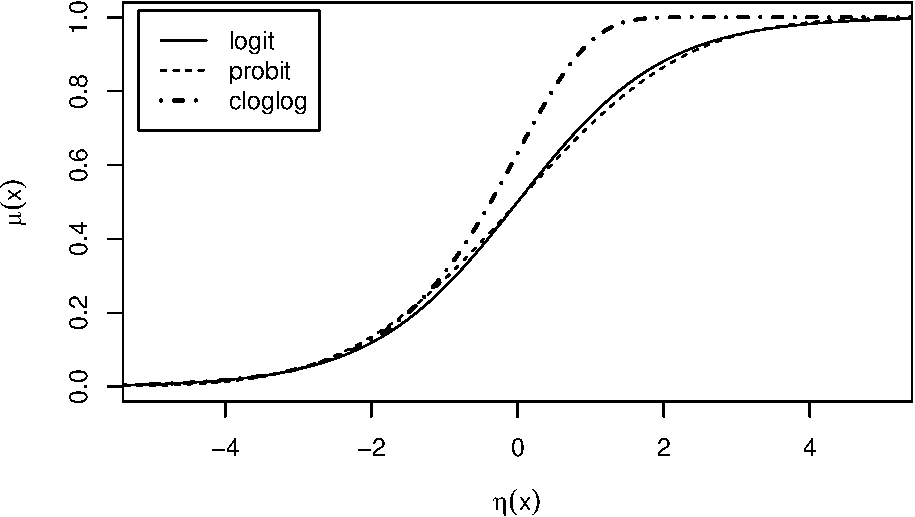
\includegraphics{LogisticRegressCh6_files/figure-latex/unnamed-chunk-2-1.pdf}

\hypertarget{example-womens-labor-force-participation}{%
\subsection{Example: Women's Labor Force
Participation}\label{example-womens-labor-force-participation}}

To illustrate logistic regression, we turn to a study of the U.S. Panel
Study of Income Dynamics of the response variable is married women's
labor force participation. The data is in Mroz (carData).
\[\begin{array}{llc}
  \bf{Variable} & {\bf Description} & {\bf Remarcs} \\
  lfp & \verb+labor force participation+ & factor: no, yes \\
  k5 & \verb+number of children ages 5 and younger+ & 0-3 \\
  k618 & \verb+number of children ages 6 to 18+ & 0-8\\
  age & \verb+wife's age in yars+ & 30-60 \\
  wc & \verb+wife's college attendance+ & factor: no, yes \\
  hc & \verb+husband's college attendance+ & factor: no, yes \\
  lwg & \verb+log of estimated wife's wage+ &  \\
  inc & \verb+family income excluding wife's income+ & 1000s
\end{array} \]

So, the estimated logistic-regression model is given by

\[log[\frac{\hat\mu(x)}{1-\hat\mu(x)}] = \beta_0 + \beta_1 x_1 + \beta_2 x_2 + \cdots + \beta_k x_k\]

If exponentiate both sides of the equation, we get
\[\frac{\hat\mu(x)}{1-\hat\mu(x)} = exp(\beta_0) \times exp(\beta_1 x_1) \times exp(\beta_2 x_2) \times \cdots \times exp(beta_k x_k)\]

where the left hand of the equation,
\(\frac{\hat\mu(x)}{1-\hat\mu(x)}\), gives the \emph{fitted odds} of
success, \textbf{the fitted probability of success divided by the fitted
probability of failure}. Exponentiating the model removes the logarithms
and changes the model in the log-odds scale to one that is
multiplicative, in this log odds scale.

\begin{Shaded}
\begin{Highlighting}[]
\CommentTok{##################### From car}
\CommentTok{# carData Mroz}
\KeywordTok{summary}\NormalTok{(Mroz)}
\end{Highlighting}
\end{Shaded}

\begin{verbatim}
  lfp            k5              k618            age          wc        hc     
 no :325   Min.   :0.0000   Min.   :0.000   Min.   :30.00   no :541   no :458  
 yes:428   1st Qu.:0.0000   1st Qu.:0.000   1st Qu.:36.00   yes:212   yes:295  
           Median :0.0000   Median :1.000   Median :43.00                      
           Mean   :0.2377   Mean   :1.353   Mean   :42.54                      
           3rd Qu.:0.0000   3rd Qu.:2.000   3rd Qu.:49.00                      
           Max.   :3.0000   Max.   :8.000   Max.   :60.00                      
      lwg               inc        
 Min.   :-2.0541   Min.   :-0.029  
 1st Qu.: 0.8181   1st Qu.:13.025  
 Median : 1.0684   Median :17.700  
 Mean   : 1.0971   Mean   :20.129  
 3rd Qu.: 1.3997   3rd Qu.:24.466  
 Max.   : 3.2189   Max.   :96.000  
\end{verbatim}

\begin{Shaded}
\begin{Highlighting}[]
\CommentTok{# logistic model family= binomial's default link is logit}
\NormalTok{mroz.mod <-}\StringTok{ }\KeywordTok{glm}\NormalTok{(lfp }\OperatorTok{~}\StringTok{ }\NormalTok{k5 }\OperatorTok{+}\StringTok{ }\NormalTok{k618 }\OperatorTok{+}\StringTok{ }\NormalTok{age }\OperatorTok{+}\StringTok{ }\NormalTok{wc }\OperatorTok{+}\StringTok{ }\NormalTok{hc }\OperatorTok{+}\StringTok{ }\NormalTok{lwg }\OperatorTok{+}\StringTok{ }\NormalTok{inc, }\DataTypeTok{family=}\NormalTok{binomial, }\DataTypeTok{data=}\NormalTok{Mroz)}
\KeywordTok{S}\NormalTok{(mroz.mod)}
\end{Highlighting}
\end{Shaded}

\begin{verbatim}
Call: glm(formula = lfp ~ k5 + k618 + age + wc + hc + lwg + inc, family =
          binomial, data = Mroz)

Coefficients:
             Estimate Std. Error z value Pr(>|z|)    
(Intercept)  3.182140   0.644375   4.938 7.88e-07 ***
k5          -1.462913   0.197001  -7.426 1.12e-13 ***
k618        -0.064571   0.068001  -0.950 0.342337    
age         -0.062871   0.012783  -4.918 8.73e-07 ***
wcyes        0.807274   0.229980   3.510 0.000448 ***
hcyes        0.111734   0.206040   0.542 0.587618    
lwg          0.604693   0.150818   4.009 6.09e-05 ***
inc         -0.034446   0.008208  -4.196 2.71e-05 ***
---
Signif. codes:  0 '***' 0.001 '**' 0.01 '*' 0.05 '.' 0.1 ' ' 1

(Dispersion parameter for binomial family taken to be 1)

    Null deviance: 1029.75  on 752  degrees of freedom
Residual deviance:  905.27  on 745  degrees of freedom

 logLik      df     AIC     BIC 
-452.63       8  921.27  958.26 

Number of Fisher Scoring iterations: 4

Exponentiated Coefficients and Confidence Bounds
              Estimate     2.5 %     97.5 %
(Intercept) 24.0982799 6.9377228 87.0347916
k5           0.2315607 0.1555331  0.3370675
k618         0.9374698 0.8200446  1.0710837
age          0.9390650 0.9154832  0.9625829
wcyes        2.2417880 1.4347543  3.5387571
hcyes        1.1182149 0.7467654  1.6766380
lwg          1.8306903 1.3689201  2.4768235
inc          0.9661401 0.9502809  0.9814042
\end{verbatim}

Exponentiating the model removes the logarithms (S function shows the
exponents of the betas). For example increasing the age of a woman by
one year, holding the other predictors constant, from
\(odds = \exp(c_0) \times \exp(c_1) \times \exp(c_2) \times \exp(\beta_3) \times \exp(c_4) \dots\)
therefore multiplies the fitted odds of her being in the workforce by
\(\exp(\beta_3) = \exp(-0.06287) = 0.9391\). That is, reduces the odds
of working by \(100(1-0.9391) \approx 6\%\). Compared to a woman that
who did not attend college, a college-educated woman with all other
predictors fixed has fitted odds of working about 2.24 times higher,
with a 95\% confidence interval {[}1.43, 3.54{]}. The exponents of the
coefficient estimates are called \emph{risk factors} or \emph{odds
ratios}. The confidence intervals for the GLM are based on profiling the
log-likelihood. The confidence intervals may not be symmetric.

\hypertarget{volunteering-for-a-psychological-experiment}{%
\subsection{Volunteering for a Psychological
Experiment}\label{volunteering-for-a-psychological-experiment}}

Cowles collected data on the willingness of students in an introductory
psychology class to volunteer for a psychological experiment. The data
set contains several variables: 1. The personality dimension
\emph{neuroticism}, a numeric variable with integer scores on a scale
from zero to 24 2. The personality dimension \emph{extraversion}, also a
numeric variable with a potential range of zero to 24. 3. The factor
sex, with levels ``female'' and ``male''. 4. Tha factor volunteer, with
levels ``no'' and ``yes''.

Researchers expected volunteering to depend on the sex variable and on
the interaction of the personality dimensions, so included the
linear-by-linear interaction between nuroticism and extraversion:

\begin{Shaded}
\begin{Highlighting}[]
\KeywordTok{brief}\NormalTok{(Cowles)}
\end{Highlighting}
\end{Shaded}

\begin{verbatim}
1421 x 4 data.frame (1416 rows omitted)
     neuroticism extraversion    sex volunteer
             [i]          [i]    [f]       [f]
1             16           13 female       no 
2              8           14 male         no 
3              5           16 male         no 
. . .                                              
1420          19           20 female       yes
1421          15           20 male         yes
\end{verbatim}

\begin{Shaded}
\begin{Highlighting}[]
\KeywordTok{sum}\NormalTok{(Cowles}\OperatorTok{$}\NormalTok{volunteer }\OperatorTok{==}\StringTok{ "yes"}\NormalTok{) }\CommentTok{# number yes}
\end{Highlighting}
\end{Shaded}

\begin{verbatim}
[1] 597
\end{verbatim}

\begin{Shaded}
\begin{Highlighting}[]
\NormalTok{cowles.mod <-}\StringTok{ }\KeywordTok{glm}\NormalTok{(volunteer }\OperatorTok{~}\StringTok{ }\NormalTok{sex }\OperatorTok{+}\StringTok{ }\NormalTok{neuroticism}\OperatorTok{*}\NormalTok{extraversion,}
    \DataTypeTok{data=}\NormalTok{Cowles, }\DataTypeTok{family=}\NormalTok{binomial)}
\KeywordTok{brief}\NormalTok{(cowles.mod, }\DataTypeTok{pvalues=}\OtherTok{TRUE}\NormalTok{)}
\end{Highlighting}
\end{Shaded}

\begin{verbatim}
              (Intercept) sexmale neuroticism extraversion
Estimate        -2.36e+00 -0.2472     0.11078     1.67e-01
Std. Error       5.01e-01  0.1116     0.03765     3.77e-02
Pr(>|t|)         2.55e-06  0.0268     0.00326     9.75e-06
exp(Estimate)    9.46e-02  0.7810     1.11715     1.18e+00
              neuroticism:extraversion
Estimate                      -0.00855
Std. Error                     0.00293
Pr(>|t|)                       0.00355
exp(Estimate)                  0.99148

 Residual deviance = 1897 on 1416 df
\end{verbatim}

\hypertarget{predictor-effect-plots-for-logistic-regression}{%
\subsection{Predictor Effect Plots for Logistic
Regression}\label{predictor-effect-plots-for-logistic-regression}}

The \textbf{effects} package, can draw predictor effect plots for
generalized linear models, including logistic regression.

\begin{Shaded}
\begin{Highlighting}[]
\KeywordTok{plot}\NormalTok{(}\KeywordTok{predictorEffects}\NormalTok{(mroz.mod))}
\end{Highlighting}
\end{Shaded}

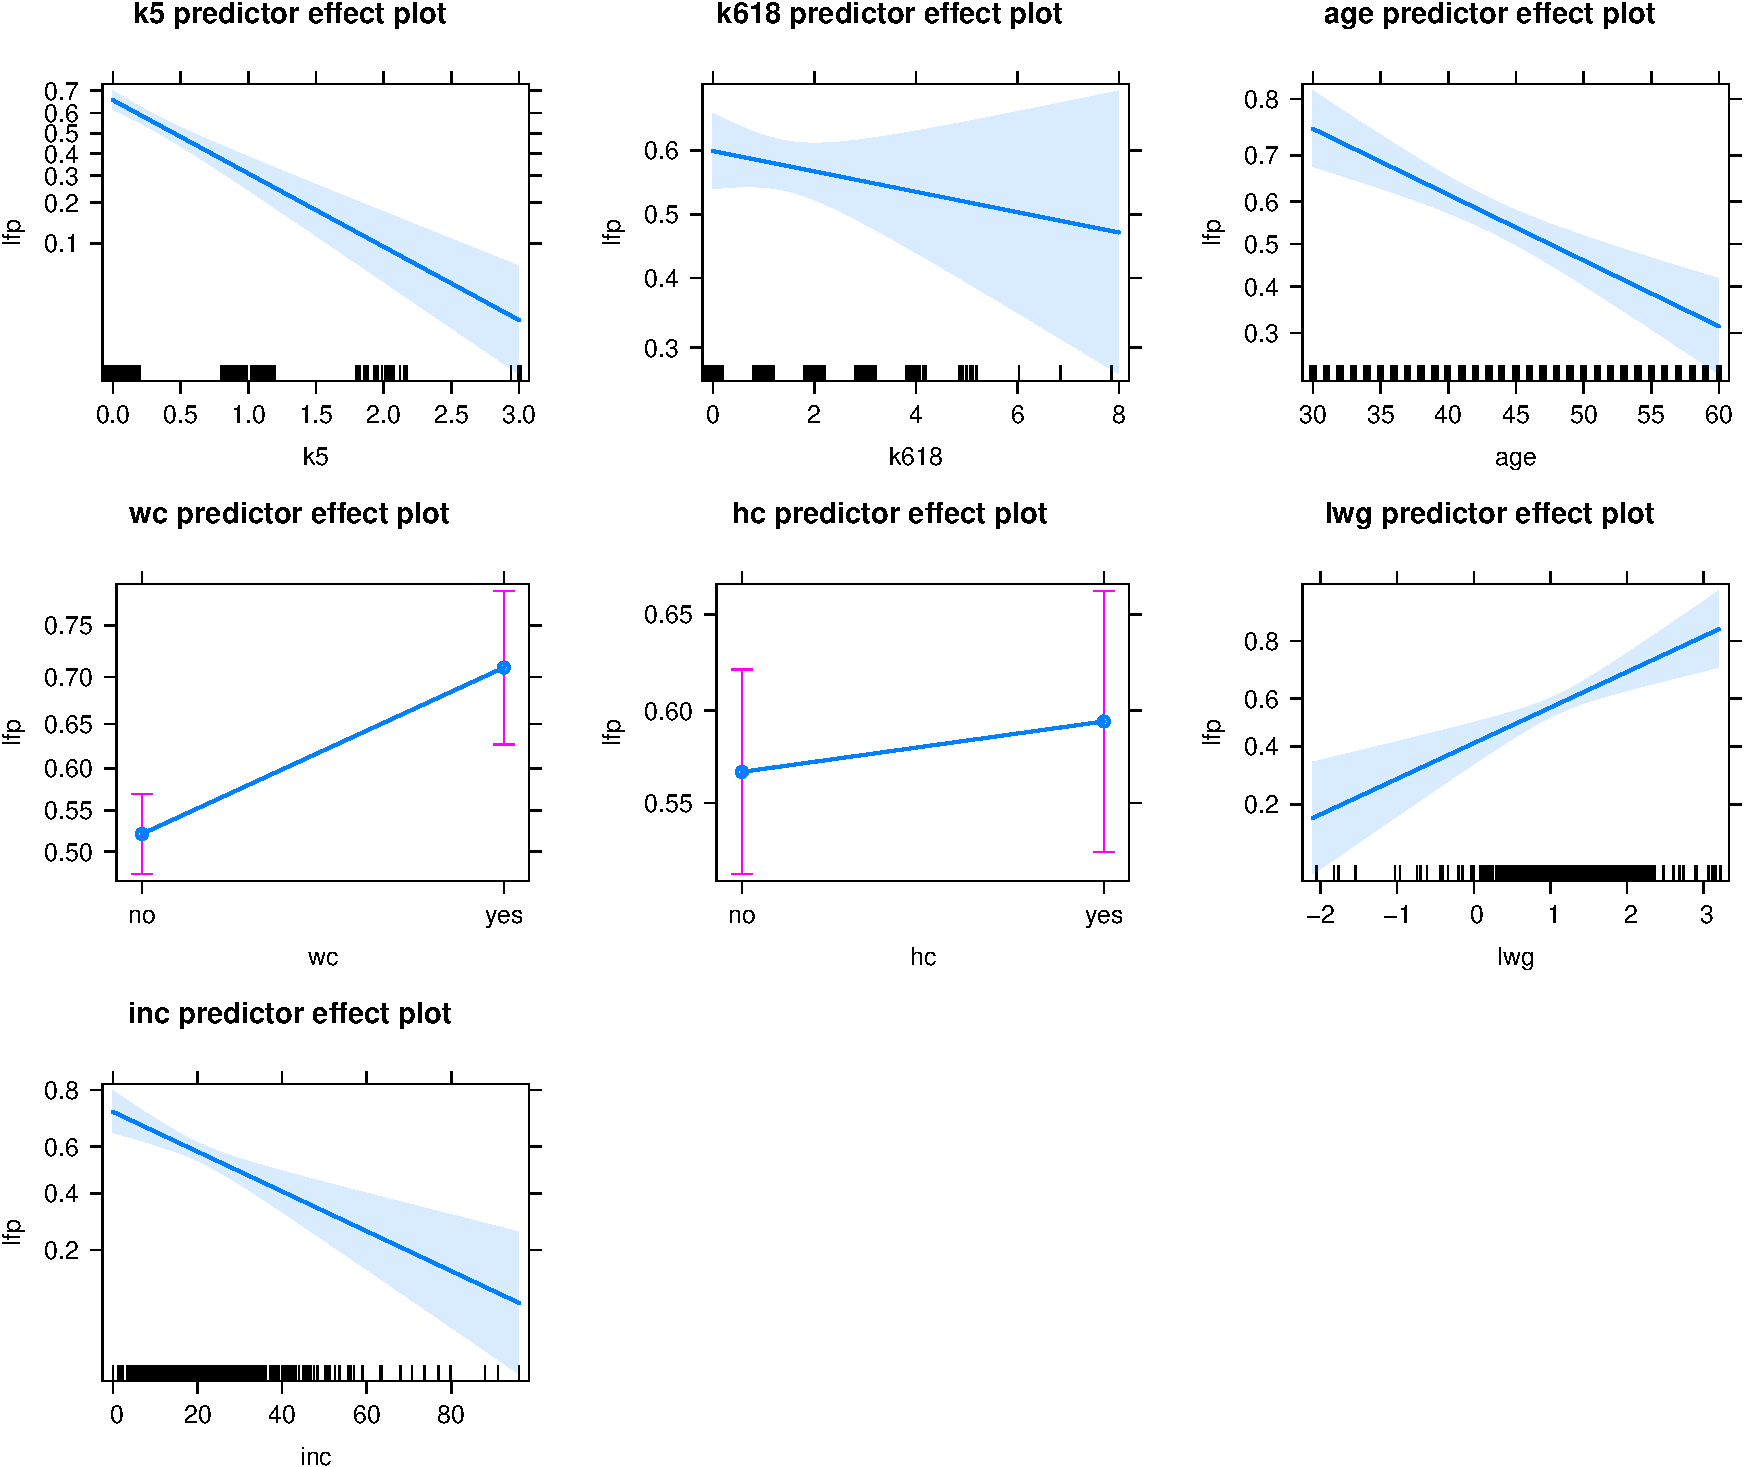
\includegraphics{LogisticRegressCh6_files/figure-latex/unnamed-chunk-5-1.pdf}

\begin{Shaded}
\begin{Highlighting}[]
\KeywordTok{plot}\NormalTok{(}\KeywordTok{predictorEffects}\NormalTok{(cowles.mod, }\OperatorTok{~}\StringTok{ }\NormalTok{neuroticism }\OperatorTok{+}\StringTok{ }\NormalTok{extraversion,}
    \DataTypeTok{xlevels=}\KeywordTok{list}\NormalTok{(}\DataTypeTok{neuroticism=}\KeywordTok{seq}\NormalTok{(}\DecValTok{0}\NormalTok{, }\DecValTok{24}\NormalTok{, }\DataTypeTok{by=}\DecValTok{8}\NormalTok{), }
        \DataTypeTok{extraversion=}\KeywordTok{seq}\NormalTok{(}\DecValTok{0}\NormalTok{, }\DecValTok{24}\NormalTok{, }\DataTypeTok{by=}\DecValTok{8}\NormalTok{))), }
    \DataTypeTok{lines=}\KeywordTok{list}\NormalTok{(}\DataTypeTok{multiline=}\OtherTok{TRUE}\NormalTok{))}
\end{Highlighting}
\end{Shaded}

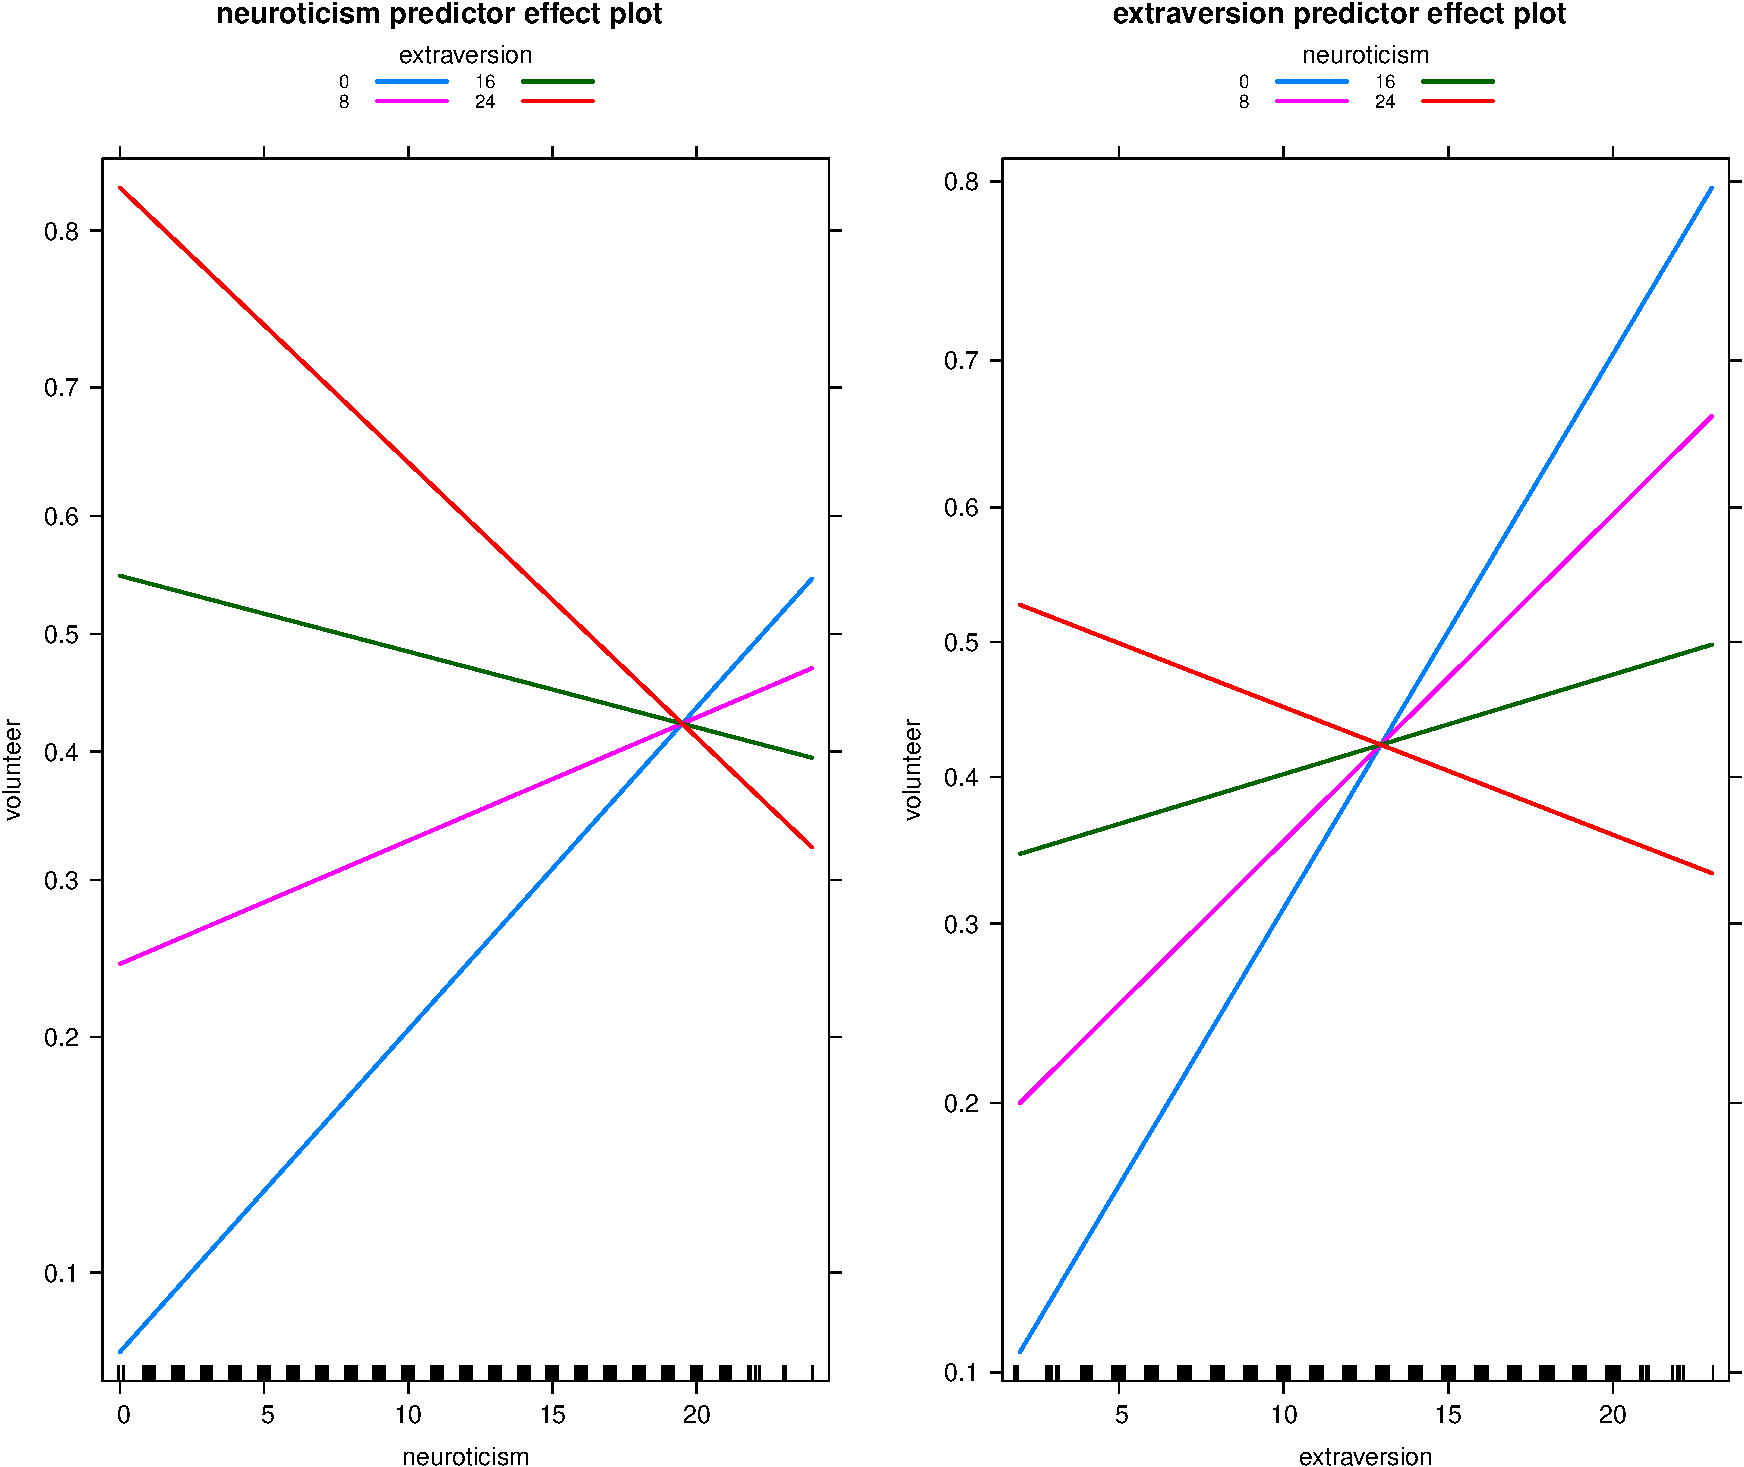
\includegraphics{LogisticRegressCh6_files/figure-latex/unnamed-chunk-5-2.pdf}

\hypertarget{analysis-of-deviance-and-hypotesis-test-for-logistic-regression}{%
\subsection{Analysis of Deviance and Hypotesis Test for Logistic
Regression}\label{analysis-of-deviance-and-hypotesis-test-for-logistic-regression}}

\hypertarget{model-comparisons}{%
\subsubsection{Model Comparisons}\label{model-comparisons}}

\begin{Shaded}
\begin{Highlighting}[]
\NormalTok{mroz.mod}\FloatTok{.2}\NormalTok{ <-}\StringTok{ }\KeywordTok{update}\NormalTok{(mroz.mod, . }\OperatorTok{~}\StringTok{ }\NormalTok{. }\OperatorTok{-}\StringTok{ }\NormalTok{k5 }\OperatorTok{-}\StringTok{ }\NormalTok{k618)}
\KeywordTok{anova}\NormalTok{(mroz.mod}\FloatTok{.2}\NormalTok{, mroz.mod, }\DataTypeTok{test=}\StringTok{"Chisq"}\NormalTok{)}
\end{Highlighting}
\end{Shaded}

\begin{verbatim}
Analysis of Deviance Table

Model 1: lfp ~ age + wc + hc + lwg + inc
Model 2: lfp ~ k5 + k618 + age + wc + hc + lwg + inc
  Resid. Df Resid. Dev Df Deviance  Pr(>Chi)    
1       747     971.75                          
2       745     905.27  2   66.485 3.655e-15 ***
---
Signif. codes:  0 '***' 0.001 '**' 0.01 '*' 0.05 '.' 0.1 ' ' 1
\end{verbatim}

\begin{Shaded}
\begin{Highlighting}[]
\KeywordTok{brief}\NormalTok{(cowles.mod}\FloatTok{.0}\NormalTok{ <-}\StringTok{ }\KeywordTok{update}\NormalTok{(cowles.mod, }
\NormalTok{    . }\OperatorTok{~}\StringTok{ }\NormalTok{. }\OperatorTok{-}\StringTok{ }\NormalTok{neuroticism}\OperatorTok{:}\NormalTok{extraversion))}
\end{Highlighting}
\end{Shaded}

\begin{verbatim}
              (Intercept) sexmale neuroticism extraversion
Estimate           -1.116  -0.235     0.00636       0.0663
Std. Error          0.249   0.111     0.01136       0.0143
exp(Estimate)       0.327   0.790     1.00638       1.0686

 Residual deviance = 1906 on 1417 df
\end{verbatim}

\begin{Shaded}
\begin{Highlighting}[]
\KeywordTok{anova}\NormalTok{(cowles.mod}\FloatTok{.0}\NormalTok{, cowles.mod, }\DataTypeTok{test=}\StringTok{"Chisq"}\NormalTok{)}
\end{Highlighting}
\end{Shaded}

\begin{verbatim}
Analysis of Deviance Table

Model 1: volunteer ~ sex + neuroticism + extraversion
Model 2: volunteer ~ sex + neuroticism * extraversion
  Resid. Df Resid. Dev Df Deviance Pr(>Chi)   
1      1417     1906.1                        
2      1416     1897.4  1   8.6213 0.003323 **
---
Signif. codes:  0 '***' 0.001 '**' 0.01 '*' 0.05 '.' 0.1 ' ' 1
\end{verbatim}

\begin{Shaded}
\begin{Highlighting}[]
\CommentTok{# Type II Tests }
\KeywordTok{Anova}\NormalTok{(mroz.mod)}
\end{Highlighting}
\end{Shaded}

\begin{verbatim}
Analysis of Deviance Table (Type II tests)

Response: lfp
     LR Chisq Df Pr(>Chisq)    
k5     66.484  1  3.527e-16 ***
k618    0.903  1   0.342042    
age    25.598  1  4.204e-07 ***
wc     12.724  1   0.000361 ***
hc      0.294  1   0.587489    
lwg    17.001  1  3.736e-05 ***
inc    19.504  1  1.004e-05 ***
---
Signif. codes:  0 '***' 0.001 '**' 0.01 '*' 0.05 '.' 0.1 ' ' 1
\end{verbatim}

\begin{Shaded}
\begin{Highlighting}[]
\KeywordTok{Anova}\NormalTok{(cowles.mod)}
\end{Highlighting}
\end{Shaded}

\begin{verbatim}
Analysis of Deviance Table (Type II tests)

Response: volunteer
                         LR Chisq Df Pr(>Chisq)    
sex                        4.9184  1   0.026572 *  
neuroticism                0.3139  1   0.575316    
extraversion              22.1372  1  2.538e-06 ***
neuroticism:extraversion   8.6213  1   0.003323 ** 
---
Signif. codes:  0 '***' 0.001 '**' 0.01 '*' 0.05 '.' 0.1 ' ' 1
\end{verbatim}

\begin{Shaded}
\begin{Highlighting}[]
\CommentTok{# Other Hypothesis Tests}
\KeywordTok{linearHypothesis}\NormalTok{(mroz.mod, }\KeywordTok{c}\NormalTok{(}\StringTok{"k5"}\NormalTok{, }\StringTok{"k618"}\NormalTok{))}
\end{Highlighting}
\end{Shaded}

\begin{verbatim}
Linear hypothesis test

Hypothesis:
k5 = 0
k618 = 0

Model 1: restricted model
Model 2: lfp ~ k5 + k618 + age + wc + hc + lwg + inc

  Res.Df Df  Chisq Pr(>Chisq)    
1    747                         
2    745  2 55.163  1.051e-12 ***
---
Signif. codes:  0 '***' 0.001 '**' 0.01 '*' 0.05 '.' 0.1 ' ' 1
\end{verbatim}

\begin{Shaded}
\begin{Highlighting}[]
\KeywordTok{linearHypothesis}\NormalTok{(mroz.mod, }\StringTok{"k5 = k618"}\NormalTok{)}
\end{Highlighting}
\end{Shaded}

\begin{verbatim}
Linear hypothesis test

Hypothesis:
k5 - k618 = 0

Model 1: restricted model
Model 2: lfp ~ k5 + k618 + age + wc + hc + lwg + inc

  Res.Df Df  Chisq Pr(>Chisq)    
1    746                         
2    745  1 49.479  2.005e-12 ***
---
Signif. codes:  0 '***' 0.001 '**' 0.01 '*' 0.05 '.' 0.1 ' ' 1
\end{verbatim}

\hypertarget{fitted-and-predicted-values}{%
\subsection{Fitted and Predicted
Values}\label{fitted-and-predicted-values}}

The function \(\verb+predict()+\) returns the estimated linear predictor
values for each observation. And to get the fitted probabilities we use
the argument type=``response''. The \(\verb+fitted()+\) function can
also be used.

\begin{Shaded}
\begin{Highlighting}[]
\NormalTok{opts <-}\StringTok{ }\KeywordTok{options}\NormalTok{(}\DataTypeTok{digits=}\DecValTok{5}\NormalTok{)}
\KeywordTok{head}\NormalTok{(}\KeywordTok{predict}\NormalTok{(mroz.mod)) }\CommentTok{# first few values}
\end{Highlighting}
\end{Shaded}

\begin{verbatim}
        1         2         3         4         5         6 
 0.063337  0.693821 -0.174106  0.672295  0.677721  0.388719 
\end{verbatim}

\begin{Shaded}
\begin{Highlighting}[]
\KeywordTok{head}\NormalTok{(}\KeywordTok{predict}\NormalTok{(mroz.mod, }\DataTypeTok{type=}\StringTok{"response"}\NormalTok{))}
\end{Highlighting}
\end{Shaded}

\begin{verbatim}
      1       2       3       4       5       6 
0.51583 0.66682 0.45658 0.66202 0.66323 0.59597 
\end{verbatim}

And the \(\verb+predict()+\) can be used to compute predicted values for
arbitrary combinations of predictor values. For example we can estimate
the probability of volunteering at neuroticism and extraversion at 12.

\begin{Shaded}
\begin{Highlighting}[]
\KeywordTok{options}\NormalTok{(opts)}

\NormalTok{predict.data <-}\StringTok{ }\KeywordTok{data.frame}\NormalTok{(}\DataTypeTok{sex=}\KeywordTok{c}\NormalTok{(}\StringTok{"female"}\NormalTok{, }\StringTok{"male"}\NormalTok{), }
    \DataTypeTok{neuroticism=}\KeywordTok{rep}\NormalTok{(}\DecValTok{12}\NormalTok{, }\DecValTok{2}\NormalTok{), }\DataTypeTok{extraversion=}\KeywordTok{rep}\NormalTok{(}\DecValTok{12}\NormalTok{, }\DecValTok{2}\NormalTok{))}
\NormalTok{predict.data}\OperatorTok{$}\NormalTok{p.volunteer <-}\StringTok{ }\KeywordTok{predict}\NormalTok{(cowles.mod, }
    \DataTypeTok{newdata=}\NormalTok{predict.data, }\DataTypeTok{type=}\StringTok{"response"}\NormalTok{)}
\NormalTok{predict.data}
\end{Highlighting}
\end{Shaded}

\begin{verbatim}
     sex neuroticism extraversion p.volunteer
1 female          12           12   0.4356968
2   male          12           12   0.3761793
\end{verbatim}

\hypertarget{binomial-data}{%
\section{Binomial Data}\label{binomial-data}}

In binomial response data, the response variable \(y_i\) for each case
\(i\) is the number of successes in a fixed number \(N_i\) of
independent trials, each with the same probability of success. Binary
regression is a limiting case of binomial regression with all the
\(N_i = 1\)

\[\begin{array}{llccc}
  \bf{\verb+Perceived Closeness+} & {\bf \verb+Intensity of Preference+} & {\bf \verb+Voted+} & {\bf \verb+ Did Not Voted+} & {\bf logit}\\
  One-sided & \verb+Weak+ & 91 & 39 & 0.847 \\
  One-sided & \verb+Medium+ & 121 & 49 & 0.904 \\
  One-sided & \verb+Strong+ & 64 & 24 & 0.981 \\
  Close & \verb+Weak+ & 214 & 87 & 0.900 \\
  Close & \verb+Medium+ & 284 & 76 & 1.318 \\
  Close & \verb+Strong+ & 201 & 25 & 2.084
\end{array} \]

\begin{Shaded}
\begin{Highlighting}[]
\NormalTok{Campbell <-}\StringTok{ }\KeywordTok{data.frame}\NormalTok{(}
    \DataTypeTok{closeness =} \KeywordTok{factor}\NormalTok{(}\KeywordTok{rep}\NormalTok{(}\KeywordTok{c}\NormalTok{(}\StringTok{"one.sided"}\NormalTok{, }\StringTok{"close"}\NormalTok{), }\KeywordTok{c}\NormalTok{(}\DecValTok{3}\NormalTok{, }\DecValTok{3}\NormalTok{)),}
        \DataTypeTok{levels=}\KeywordTok{c}\NormalTok{(}\StringTok{"one.sided"}\NormalTok{, }\StringTok{"close"}\NormalTok{)),}
    \DataTypeTok{preference =} \KeywordTok{factor}\NormalTok{(}\KeywordTok{rep}\NormalTok{(}\KeywordTok{c}\NormalTok{(}\StringTok{"weak"}\NormalTok{, }\StringTok{"medium"}\NormalTok{, }\StringTok{"strong"}\NormalTok{), }\DecValTok{2}\NormalTok{),}
        \DataTypeTok{levels=}\KeywordTok{c}\NormalTok{(}\StringTok{"weak"}\NormalTok{, }\StringTok{"medium"}\NormalTok{, }\StringTok{"strong"}\NormalTok{)),}
    \DataTypeTok{voted =} \KeywordTok{c}\NormalTok{(}\DecValTok{91}\NormalTok{, }\DecValTok{121}\NormalTok{, }\DecValTok{64}\NormalTok{, }\DecValTok{214}\NormalTok{, }\DecValTok{284}\NormalTok{, }\DecValTok{201}\NormalTok{),}
    \DataTypeTok{did.not.vote =} \KeywordTok{c}\NormalTok{(}\DecValTok{39}\NormalTok{, }\DecValTok{49}\NormalTok{, }\DecValTok{24}\NormalTok{, }\DecValTok{87}\NormalTok{, }\DecValTok{76}\NormalTok{, }\DecValTok{25}\NormalTok{)}
\NormalTok{)}
\NormalTok{Campbell}
\end{Highlighting}
\end{Shaded}

\begin{verbatim}
  closeness preference voted did.not.vote
1 one.sided       weak    91           39
2 one.sided     medium   121           49
3 one.sided     strong    64           24
4     close       weak   214           87
5     close     medium   284           76
6     close     strong   201           25
\end{verbatim}

For binomial data, the response can be the \emph{proportion} of
successes for each observation, or the proportion of successes for
failures. For example the logit for the One-sided, weak case 91 voted,
and 39 did not voted, \(\log(\verb+Voted/Did not Voted+) = \log(91/39)\)
-\textgreater{} \emph{0.847}

\begin{Shaded}
\begin{Highlighting}[]
\NormalTok{campbell.mod <-}\StringTok{ }\KeywordTok{glm}\NormalTok{(}\KeywordTok{cbind}\NormalTok{(voted, did.not.vote) }\OperatorTok{~}
\StringTok{    }\NormalTok{closeness}\OperatorTok{*}\NormalTok{preference, }\DataTypeTok{family=}\NormalTok{binomial, }\DataTypeTok{data=}\NormalTok{Campbell)}
\CommentTok{# the estimated responses are exact and the residuals are zero}
\KeywordTok{predict}\NormalTok{(campbell.mod)}
\end{Highlighting}
\end{Shaded}

\begin{verbatim}
        1         2         3         4         5         6 
0.8472979 0.9039702 0.9808293 0.9000679 1.3182409 2.0844291 
\end{verbatim}

\begin{Shaded}
\begin{Highlighting}[]
\KeywordTok{residuals}\NormalTok{(campbell.mod)}
\end{Highlighting}
\end{Shaded}

\begin{verbatim}
[1] 0 0 0 0 0 0
\end{verbatim}

\begin{Shaded}
\begin{Highlighting}[]
\KeywordTok{plot}\NormalTok{(}\KeywordTok{predictorEffects}\NormalTok{(campbell.mod, }\OperatorTok{~}\StringTok{ }\NormalTok{preference),  }
     \DataTypeTok{main=}\StringTok{""}\NormalTok{, }\DataTypeTok{confint=}\KeywordTok{list}\NormalTok{(}\DataTypeTok{style=}\StringTok{"bars"}\NormalTok{), }\DataTypeTok{lines=}\KeywordTok{list}\NormalTok{(}\DataTypeTok{multiline=}\OtherTok{TRUE}\NormalTok{),}
     \DataTypeTok{xlab=}\StringTok{"Intensity of Preference"}\NormalTok{, }\DataTypeTok{ylab=}\StringTok{"Probability of Voting"}\NormalTok{,}
     \DataTypeTok{lattice=}\KeywordTok{list}\NormalTok{(}\DataTypeTok{key.args =} \KeywordTok{list}\NormalTok{(}\DataTypeTok{x =}\FloatTok{0.1}\NormalTok{, }\DataTypeTok{y =} \FloatTok{0.95}\NormalTok{, }\DataTypeTok{corner=}\KeywordTok{c}\NormalTok{(}\DecValTok{0}\NormalTok{, }\DecValTok{1}\NormalTok{))))}
\end{Highlighting}
\end{Shaded}

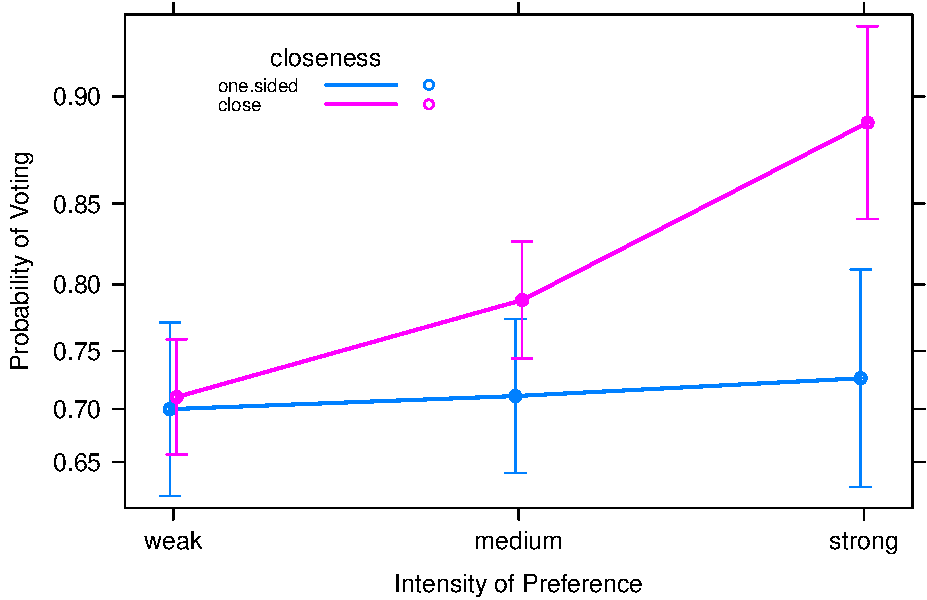
\includegraphics{LogisticRegressCh6_files/figure-latex/unnamed-chunk-10-1.pdf}

The emmeans function can be used to test differences between the two
levels of closeness fo each level of preference:

\begin{Shaded}
\begin{Highlighting}[]
\KeywordTok{emmeans}\NormalTok{(campbell.mod, pairwise }\OperatorTok{~}\StringTok{ }\NormalTok{closeness }\OperatorTok{|}\StringTok{ }\NormalTok{preference)}\OperatorTok{$}\NormalTok{contrasts}
\end{Highlighting}
\end{Shaded}

\begin{verbatim}
preference = weak:
 contrast          estimate    SE  df z.ratio p.value
 one.sided - close  -0.0528 0.230 Inf -0.230  0.8184 

preference = medium:
 contrast          estimate    SE  df z.ratio p.value
 one.sided - close  -0.4143 0.213 Inf -1.945  0.0517 

preference = strong:
 contrast          estimate    SE  df z.ratio p.value
 one.sided - close  -1.1036 0.320 Inf -3.451  0.0006 

Results are given on the log odds ratio (not the response) scale. 
\end{verbatim}

\end{document}
